\documentclass[]{LASPreport}


\newcommand{\SubSystem}{ADCS}
\newcommand{\SERnumber}{SPICE Unit Test}
\newcommand{\AgileRevisionNumber}{N/A}
\newcommand{\subject}{Unit Test Results for SPICE Interface Model}
\newcommand{\status}{Initial Test Results}
\newcommand{\preparer}{S. Piggott}
\newcommand{\summary}{
   This is a report documenting the results of the SPICE unit test created for 
   the AVS Basilisk Simulation as part of the EMM project. }


\begin{document}


\makeCover


%
%	enter the revision documentation here
%	to add more lines, copy the table entry and the \hline, and paste after the current entry.
%
\pagestyle{empty}
{\renewcommand{\arraystretch}{2}
\noindent
\begin{longtable}{|p{0.5in}|p{4.5in}|p{1.14in}|}
\hline
{\bfseries Rev}: & {\bfseries Change Description} & {\bfseries By} \\
\hline
Draft & Initial Revision & S. Piggott \\
\hline

\end{longtable}
}

\newpage
\setcounter{page}{1}
\pagestyle{fancy}

\tableofcontents
~\\ \hrule ~\\

%\begin{figure}[htb]
%	\centerline{
%	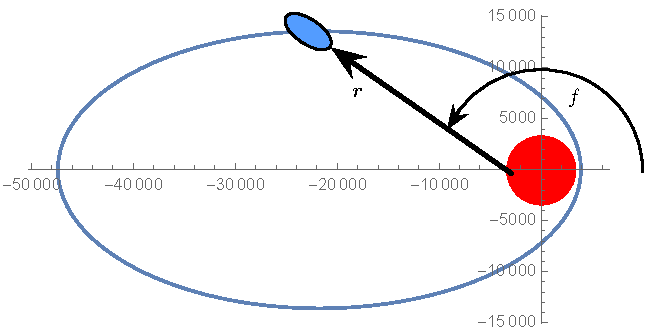
\includegraphics[]{Figures/Fig1}
%	}
%	\caption{Sample Figure Inclusion.}
%	\label{fig:Fig1}
%\end{figure}

\section{Introduction}
The SPICE Interface model in the AVS Basilisk simulation is used to generate 
information on what the overal universal time is (ex. UTC/UT1/etc) as well as 
ephemeris information for planetary bodies such as Mars, Earth, and the Sun.  
The time functionality of the model is required for the simulation because we 
must be able to input specific starting epochs as well as output accurate time 
tags in a format usable by others on the project.  The planetary ephemeris 
information is required because we need to be able to compute the location of 
the various planetary bodies in order to simulate the effects of their gravity 
on the spacecraft.


\section{Test Design}
The unit test for the spice\_interface module is located in:\\

\noindent
{\tt SimCode/environment/spice/UnitTest/SpiceUnitTest.py \\
\\

\noindent This unit test is designed to functionally test the simulation model 
outputs as well as get complete code path coverage.  The test design is broken 
up into several parts:\\
\begin{enumerate}
\item{Time Increment Check: The simulation is advanced at a fixed rate and all 
   of the increments are checked to ensure that they are consistent.}
\item{Absolute Time Check: The simulation-computed GPS time at a specific UTC 
  time is checked to ensure that it is correct with respect to the true value 
  of GPS time for that UTC epoch.}
\item{Julian Date Time Check: The simulated Julian Date time is compared for the 
   same UTC epoch used for the previous test.}
\item{Mars Position Check: The computed position of Mars in the inertial frame 
   is compared against a value taken for Mars from the JPL Horizons ephemeris 
   system for the same epoch time.}
\item{Earth Position Check: The computed position of Earth in the inertial frame 
   is compared against a value taken for Earth from the JPL Horizons ephemeris 
   system for the same epoch time.}
\item{Sun Position Check: The computed position of Sun in the inertial frame 
   is compared against a value taken for Sun from the JPL Horizons ephemeris 
   system for the same epoch time.}
\end{enumerate}


\section{Test Results}
\begin{enumerate}
\item{Time Increment Check: The difference between the increments was checked 
   to make sure that it was less than 1.0 microseconds which is less than our 
   required time accuracy.  Check successful.}
\item{Absolute Time Check: The difference between the truth GPS time at the UTC 
   epoch (2016 June 16, 00:00:00.0 TDB) was within 1.0 microseconds of the 
   simulated value.  Check successsful.}
\item{Julian Date Time Check: The truth Julian date was within 0.1 seconds of 
   the simulated Julian date which is near the precision of the Julian Date 
   computation accuracy.  Check successful.}
\item{Mars Position Check:  The Position of Mars from the Horizons ephemeris 
   system only agreed with the simulation output to 1626 meters.  This is above 
   the success criteria for the test.  \textcolor{red}{Check failed.}}
\item{Earth Position Check:  The Position of Earth from the Horizons ephemeris 
   system only agreed with the simulation output to 1626 meters.  This is above 
   the success criteria for the test.  \textcolor{red}{Check failed.}}
\item{Sun Position Check: The Position of the Sun from the Horizons ephemeris 
   system was within 800 m of the simulated output.  This meets the success 
   criteria for the test although it is believed that there are issues with the 
   Sun similar to the Mars/Earth tests. Check successful.}
\end{enumerate}

\section{Test Coverage}
The method coverage for all of the methods included in the spice\_interface 
module are tabulated in Table~\ref{tab:cov_met}

\begin{table}[htbp]
    \caption{Test Analysis Results}
   \label{tab:cov_met}
        \centering \fontsize{10}{10}\selectfont
   \begin{tabular}{c | r | r | r} % Column formatting, 
      \hline
      Method Name    & Unit Test Coverage (\%) & Runtime Self (\%) & Runtime Children (\%) \\
      \hline
      UpdateState & 100.0 & 0.03 & 24.2 \\
      loadSpiceKernel & 100.0 & 0.0 & 0.0 \\
      SelfInit & 100.0 & 0.0 & 0.0 \\
      InitTimeData & 100.0 & 0.0 & 0.0 \\
      ComputeGPSData & 100.0 & 0.0 & 0.0 \\
      ComputePlanetData & 100.0 & 0.18 & 13.26 \\
      SendOutputData & 100.0 & 0.0 & 0.0 \\
      \hline
   \end{tabular}
\end{table}

For all of the methods in the spice\_interface modules, the code coverage 
percentage is 100\% which meets our test requirements.  The CPU usage drawn by 
the module is one of the highest percents in the entire test (24\%).  This is 
being almost entirely driven by external components (JPL's SPICE and boost).  
We could certainly look at building those modules with optimization to cut 
down the CPU usage, or even call this module at a lower rate with another 
module added to maintain the times/states at high rate.

\section{Conclusions}
The spice\_interface module requires further work.  We need to go and investigate 
why the planetary ephemeris computations are different from what we obtained 
from the Horizons system.  In all actuality those results are fine, but we do 
need to go and figure out why the difference exists.  It could be a hidden time 
error or other small effect that could impact our analysis going forward.  
However, it is close enough that we can definitely proceed with PDR analysis 
using the model as is.

\end{document}
